\subsection{Representations of Variability Models}

\begin{frame}{\myframetitle}
	% this notation is already nice for communication, but semantics matter (for large models, it does not suffice to look sharply)
	% why is this needed? (forward ref?)
	% this section shall teach the relationship between FMs and formulas and FMs and sets (i.e., Damiani 2020, Batory 2005), so: FM semantics
	% also, (valid) total configurations should be explained here (how a computer can check them, this can be checked easily when an FM is encoded eg as runtime variability, but all other SAT-based questions are hard to answer)

	\begin{mycolumns}
		\myexample{Natural Language}{
			\tiny ``A \feat{configurable database} has an API that allows for at least one of the request types \feat{Get}, \feat{Put}, or \feat{Delete}.
			Optionally, the database can support \feat{transactions}, provided that the API allows for Put or Delete requests.
			Also, the database targets a supported operating system, which is either \feat{Windows} or \feat{Linux}.''
		}
		\myexample{Configuration Map}{
			\tiny
			\leftandright{
				$\{C,G,W\}$\\
				\hspace{4mm}\vdots\\[1ex]
				$\{C,G,P,D,T,W\}$
			}{
				$\{C,G,L\}$\\
				\hspace{4mm}\vdots\\[1ex]
				$\{C,G,P,D,T,L\}$
			}
		}
		\myexampletight{Feature Model}{
			\centering\tiny
			\featureDiagramConfigurableDatabase
		}
	\mynextcolumn
		\centering
		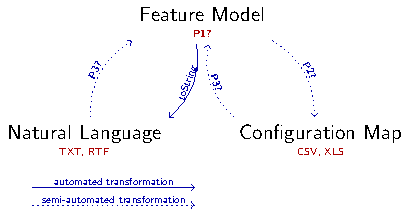
\includegraphics[width=\linewidth]{representations-high-level}

		\mynote{Problems}{
			\begin{enumerate}
				\item[P1] How to express feature models \emph{textually}? % animate P1 with arrows, see lego example
				\item[P2] How to obtain valid configurations \emph{automatically}?
				\item[P3] \color{gray}{(How to reverse engineer feature models?)}
			\end{enumerate}
		}
	\end{mycolumns}
\end{frame}

\subsection{Universal Variability Language}

\begin{frame}[fragile]{\myframetitle}
	\begin{mycolumns}
\begin{uvl}[basicstyle=\normalsize]
features
	ConfigDB
		mandatory
			API {abstract}
				or
					Get
					Put
					Delete

		optional
			Transactions
		mandatory
			OS {abstract}
				alternative
					Windows
					Linux

constraints
	Transactions => Put | Delete
\end{uvl}
	\mynextcolumn
		\myexampletight{A Feature Model ``Sideways''}{
			\centering
			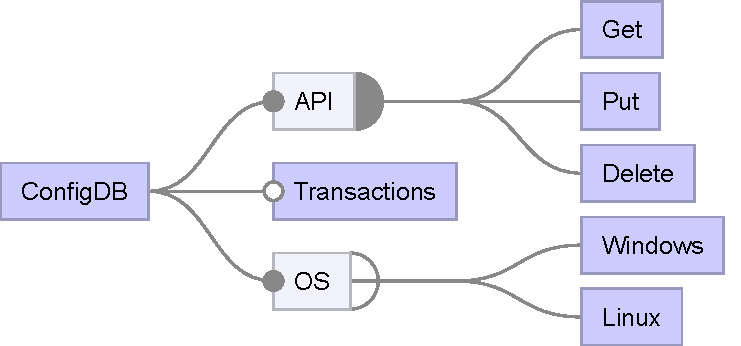
\includegraphics[width=\linewidth]{varied-model}
			$Transactions \pimplies Put \por Delete$
		}
		\mynote{Universal Variability Language (UVL)}{
			\begin{itemize}
				\item textual language for feature modeling
				\item adds advanced modeling constructs (e.g., attributes, cardinalities, submodels, \ldots)
			\end{itemize}
		}
	\end{mycolumns}
\end{frame}

\begin{frame}{} %todo good name
	\centering
	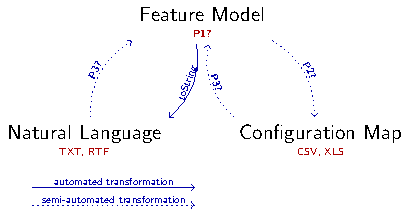
\includegraphics[width=0.45\linewidth]{representations-high-level}
	\begin{mycolumns}[animation=none]
		\mynote{Problems}{
			\begin{enumerate}
				\item[P1] How to express feature models \emph{textually}?
				\item[P2] How to obtain valid configurations \emph{automatically}?
				\item[P3] \color{gray}{(How to reverse engineer feature models?)}
			\end{enumerate}
		}
		\mynextcolumn
		\mynote{Solutions}{
			\begin{enumerate}
				\item[P1] Universal Variability Language $\rightarrow$ \emph{Syntax}
				\item[P2] \emph{Semantics}?
				\item[P3] \color{gray}{--}
			\end{enumerate}
		}
	\end{mycolumns}
\end{frame}

\subsection{Recap: Propositional Formulas}

\begin{frame}{\myframetitle}
	\begin{mycolumns}
		\mydefinition{Syntax of Propositional Formulas}{
			Inductive definition of \emph{(propositional) formulas}\\\deutsch{(aussagenlogische) Formeln}:
			\begin{itemize}
				\item the \emph{(Boolean) truth values} $\top$, $\bot$
				\item any \emph{(Boolean) variable} $X$
    			\item any \emph{negation} $\pnot \phi$ of a formula $\phi$
    			\item any \emph{conjunction} $(\phi \pand \psi)$ of formulas $\phi$ and $\psi$
				\item any \emph{disjunction} $(\phi \por \psi)$, \emph{implication} $(\phi \pimplies \psi)$, or \emph{biimplication} $(\phi \pequals \psi)$
			\end{itemize}
		}
		\mynote{Operator Precedence: $\pnot$, $\pand$, $\por$, $\pimplies$, $\pequals$}{
			\vspace*{-4ex} % TODO Benno: why is this hack needed?
			\begin{align*}
				           &~Transactions \pimplies (Put \por Delete) \\
				\equiv     &~Transactions \pimplies Put \por Delete \\
				\not\equiv &~(Transactions \pimplies Put) \por Delete
			\end{align*}
		}
	\mynextcolumn
		\mydefinition{Informal Semantics of Propositional Formulas}{
			\vspace*{-4ex}
			\begin{equation*}
				\begin{rcases}
					\top                \\
					\bot                \\
					\pnot \phi          \\
					\phi \pand \psi     \\
					\phi \por \psi      \\
					\phi \pimplies \psi \\
					\phi \pequals \psi
				\end{rcases} \text{ means } \begin{cases}
					\text{``true'' (or \emph{tautology})} \\
					\text{``false'' (or \emph{contradiction})} \\
					\text{``not $\phi$''} \\
					\text{``$\phi$ and $\psi$''} \\
					\text{``$\phi$ or $\psi$'' (inclusive or!)} \\
					\text{``if $\phi$, then $\psi$'' (and else?)} \\
					\text{``$\phi$ if and only if $\psi$''}
				\end{cases}
			\end{equation*}
		}
		\mynote{Differences to First-Order Logic}{
			\begin{itemize}
				\item no quantifiers $\forall, \exists$
    			\item no predicates $P(\ldots)$ (e.g., $=$, $>$, $isA$)
    			\item no functions $f(\ldots)$ (e.g., $+$, $\ast$, $typeOf$)
				\item no constants (e.g., $42$, ``hello'')
			\end{itemize}
		}
	\end{mycolumns}
\end{frame}

\subsection{From Feature Model to Formula}

\subsubsection{Example}

\begin{frame}{\myframetitle}
	\begin{mycolumns}[animation=none]
		\only<1-|handout:1-2>{
			\myexampletight{A Feature Model $FM$ \ldots}{
				\centering\tiny
				\featureDiagramConfigurableDatabase[_phi]
				\featureDiagramOverlay{
					\only<1|handout:0>{
						\featureDeemph{(API_phi),(Get_phi),(Put_phi),(Delete_phi),(Transactions_phi),(OS_phi),(Windows_phi),(Linux_phi)}
						\featureEmph{(ConfigDB_phi)}
					}
					\only<2|handout:0>{
						\featureDeemph{(Get_phi),(Put_phi),(Delete_phi),(Transactions_phi),(OS_phi),(Windows_phi),(Linux_phi)}
						\featureEmph{(ConfigDB_phi)(API_phi)}
					}
					\only<3|handout:0>{
						\featureDeemph{(Get_phi),(Put_phi),(Delete_phi),(API_phi),(OS_phi),(Windows_phi),(Linux_phi)}
						\featureEmph{(ConfigDB_phi)(Transactions_phi)}
					}
					\only<4|handout:0>{
						\featureDeemph{(Get_phi),(Put_phi),(Delete_phi),(API_phi),(Transactions_phi),(Windows_phi),(Linux_phi)}
						\featureEmph{(ConfigDB_phi)(OS_phi)}
					}
					\only<5|handout:0>{
						\featureDeemph{(ConfigDB_phi),(Transactions_phi),(Windows_phi),(Linux_phi),(OS_phi)}
						\featureEmph{(Get_phi)(Put_phi)(Delete_phi)(API_phi)}
					}
					\only<6-7|handout:0>{
						\featureDeemph{(Get_phi),(Put_phi),(Delete_phi),(API_phi),(Transactions_phi),(ConfigDB_phi)}
						\featureEmph{(Windows_phi)(Linux_phi)(OS_phi)}
					}
					\only<8|handout:0>{
						\featureDeemph{(ConfigDB_phi)(Transactions_phi)(Windows_phi)(Linux_phi)(OS_phi)(Get_phi)(Put_phi)(Delete_phi)(API_phi)}
					}
					\only<9-12|handout:1>{
						\featureSelected{(ConfigDB_phi),(API_phi),(Get_phi),(OS_phi),(Windows_phi)}
						\featureDeselected{(Put_phi)(Delete_phi),(Transactions_phi),(Linux_phi)}
					}
					\only<13-|handout:2>{
						\featureSelected{(ConfigDB_phi),(API_phi),(Get_phi)}
						\featureDeselected{(Put_phi)(Delete_phi)(Windows_phi)(Linux_phi),(Transactions_phi)(OS_phi)}
					}
				}
			}
			\myexample{\ldots as a Propositional Formula $\phi(FM)$}{
				\vspace*{-4ex}
				\small
				\begin{align*}
					\phi(FM) = &~ConfigDB \\
					\uncover<2->{\pand &~(API \pequals ConfigDB) \\}
					\uncover<3->{\pand &~(Transactions \pimplies ConfigDB) \\}
					\uncover<4->{\pand &~(OS \pequals ConfigDB) \\}
					\uncover<5->{\pand &~(Get \por Put \por Delete \pequals API) \\}
					\uncover<6->{\pand &~(Windows \por Linux \pequals OS) \\}
					\uncover<7->{\pand &~\pnot (Windows \pand Linux) \\}
					\uncover<8->{\pand &~(Transactions \pimplies Put \por Delete)}
				\end{align*}
			}
		}
	\mynextcolumn
		\only<9-|handout:1-2>{
			\myexample{Is This a Valid Configuration?}{
				\vspace*{-4ex}
				\only<9-12|handout:1>{
					\begin{align*}
								&~\phi(FM)({\{C, A, G, O, W\}}) \\
						=		&~\phi(FM)(\cfg[2-]{C, A, G, O, W}{P, D, T, L}) \\
						\uncover<10->{=&~\fs{C} \pand (\fs{A} \pequals \fs{C}) \pand (\fd{T} \pimplies \fs{C}) \pand (\fs{O} \pequals \fs{C}) \\
						\pand &~(\fs{G} \por \fd{P} \por \fd{D} \pequals \fs{A}) \pand (\fs{W} \por \fd{L} \pequals \fs{O}) \\
						\pand &~\pnot (\fs{W} \pand \fd{L}) \pand (\fd{T} \pimplies \fd{P} \por \fd{D}) \\}
						\uncover<11->{=&~\fs{\top} \pand (\fs{\top} \pequals \fs{\top}) \pand (\fd{\bot} \pimplies \fs{\top}) \pand (\fs{\top} \pequals \fs{\top}) \\
						\pand &~(\fs{\top} \por \fd{\bot} \por \fd{\bot} \pequals \fs{\top}) \pand (\fs{\top} \por \fd{\bot} \pequals \fs{\top}) \\
						\pand &~\pnot (\fs{\top} \pand \fd{\bot}) \pand (\fd{\bot} \pimplies \fd{\bot} \por \fd{\bot}) \\}
						\uncover<12->{=&~\fs{\top} \pand \fs{\top} \pand \fs{\top} \pand \fs{\top} \pand \fs{\top} \pand \fs{\top} \pand \fs{\top} \pand \fs{\top} \\
						=		&~\fs{\top}}
					\end{align*}
					\uncover<12->{\emph{$\leadsto$ configuration is valid}\\
					\phantom{$\leadsto$ }(read-only database on Windows)}
				}
				\only<13-|handout:2>{
					\begin{align*}
								&~\phi(FM)({\{C, A, G\}}) \\
						=		&~\phi(FM)(\cfg[2-]{C, A, G}{P, D, T, O, W, L}) \\
						\uncover<14->{=&~\fs{C} \pand (\fs{A} \pequals \fs{C}) \pand (\fd{T} \pimplies \fs{C}) \pand (\fd{O} \pequals \fs{C}) \\
						\pand &~(\fs{G} \por \fd{P} \por \fd{D} \pequals \fs{A}) \pand (\fd{W} \por \fd{L} \pequals \fd{O}) \\
						\pand &~\pnot (\fd{W} \pand \fd{L}) \pand (\fd{T} \pimplies \fd{P} \por \fd{D}) \\}
						\uncover<15->{=&~\fs{\top} \pand (\fs{\top} \pequals \fs{\top}) \pand (\fd{\bot} \pimplies \fs{\top}) \pand (\fd{\bot} \pequals \fs{\top}) \\
						\pand &~(\fs{\top} \por \fd{\bot} \por \fd{\bot} \pequals \fs{\top}) \pand (\fd{\bot} \por \fd{\bot} \pequals \fd{\bot}) \\
						\pand &~\pnot (\fd{\bot} \pand \fd{\bot}) \pand (\fd{\bot} \pimplies \fd{\bot} \por \fd{\bot}) \\}
						\uncover<16->{=&~\fs{\top} \pand \fs{\top} \pand \fs{\top} \pand \fd{\bot} \pand \fs{\top} \pand \fs{\top} \pand \fs{\top} \pand \fs{\top} \\
						=		&~\fd{\bot}} % todo: only show \pand and phi(fm) = and parentheses at the end
					\end{align*}
					\uncover<16->{\emph{$\leadsto$ configuration is invalid}\\
					\phantom{$\leadsto$ }($\lightning$ no operating system)}
				}
			}
		}
	\end{mycolumns}
\end{frame}

\subsection{From Feature Model to Formula}

\subsubsection{Algorithm}

\newcommand{\featureDiagramFn}[4]{#1\left(~\parbox{#2}{\centering\scalebox{0.8}{\featureDiagram{#3}}}~\right) &= #4}
\newcommand{\featureDiagramPhantom}[4]{\vphantom{#1\left(~\parbox{#2}{\centering\scalebox{0.8}{\featureDiagram{#3}}}~\right)}}

\begin{frame}{\myframetitle}
	\begin{mycolumns}[animation=none]
		\mydefinition{}{
			\vspace*{-4ex}
			\begin{align*}
				\uncover<1->{\featureDiagramFn{\phi}{6ex}{Root,concrete}{Root}}\\
				\uncover<2->{\featureDiagramFn{\phi}{6ex}{P,concrete[C,optional,concrete]}{C \pimplies P}}\\
				\uncover<3->{\featureDiagramFn{\phi}{6ex}{P,concrete[C,mandatory,concrete]}{C \pequals P}}\\
				\uncover<4->{\featureDiagramFn{\phi}{15ex}{P,concrete[$C_1$,or,concrete][\ldots][$C_n$,concrete]}{\bigvee_{1 \leq i \leq n} C_i \pequals P}}\\
				\uncover<5->{\featureDiagramFn{\phi}{15ex}{P,concrete[$C_1$,or,concrete][\ldots][$C_n$,concrete]}{\bigvee_{1 \leq i \leq n} C_i \pequals P}}\\
				& \uncover<5->{\pand \bigwedge_{1 \leq i < j \leq n} \pnot (C_i \pand C_j)}
			\end{align*}
		}
	\mynextcolumn
	\mynote{}{
		\begin{itemize}
			\item<1-> \emph{Root feature}: $R$ is always required
   			\item<2-> \emph{Optional feature}: $C$ requires $P$
   			\item<3-> \emph{Mandatory feature}: Optional + $P$ requires $C$
   			\item<4-> \emph{Or group}: Optional + $P$ requires at least one $C_i$
   			\item<5-> \emph{Alternative group}: Optional + $P$ requires exactly one $C_i$
      % conjunction of everything
	  % cross-tree constraints
		\end{itemize}
	}
	\end{mycolumns}
\end{frame}

\subsection{Storing Formulas}

\begin{frame}{\myframetitle}
	% cnf + transf. + dimacs on one slide
	%CNF is a universal language for saving Boolean formulas, maybe explain it here?

	\begin{mycolumns}
		\mydefinition{Recap: Conjunctive Normal Form}{
			\begin{itemize}
				\item a \emph{literal} $L$ is a variable $X$ or its negation $\pnot X$
				\item a \emph{clause} $C$ is a disjunction of literals $\bigvee_{j} L_j$
				\item a \emph{conjunctive normal form (CNF)} is a conjunction of clauses $\bigwedge_{i} C_i = \bigwedge_{i} \bigvee_{j} L_j$
				\item intuitively: a set of ``rules'' to be satisfied
				\item any formula $\phi$ can be transformed into a CNF $\phi'$ that is logically equivalent ($\phi \mequals \phi'$)
			\end{itemize}
		} % later on allsat: DNF as opposition? subtractive/additive definition?
		\mydefinition{Recap: Identities}{
			\begin{itemize}
				\item 
			\end{itemize}
		}
	\mynextcolumn
		% \myexample{}{
		% 	\vspace*{-4ex}
		% 	\small
		% 	\begin{align*}
		% 		&~\phi(FM) \\
		% 		\uncover<10->{=&~\fs{C} \pand (\fs{A} \pequals \fs{C}) \pand (\fd{T} \pimplies \fs{C}) \pand (\fs{O} \pequals \fs{C}) \\
		% 		\pand &~(\fs{G} \por \fd{P} \por \fd{D} \pequals \fs{A}) \pand (\fs{W} \por \fd{L} \pequals \fs{O}) \\
		% 		\pand &~\pnot (\fs{W} \pand \fd{L}) \pand (\fd{T} \pimplies \fd{P} \por \fd{D}) \\}
		% 		\uncover<11->{=&~\fs{\top} \pand (\fs{\top} \pequals \fs{\top}) \pand (\fd{\bot} \pimplies \fs{\top}) \pand (\fs{\top} \pequals \fs{\top}) \\
		% 		\pand &~(\fs{\top} \por \fd{\bot} \por \fd{\bot} \pequals \fs{\top}) \pand (\fs{\top} \por \fd{\bot} \pequals \fs{\top}) \\
		% 		\pand &~\pnot (\fs{\top} \pand \fd{\bot}) \pand (\fd{\bot} \pimplies \fd{\bot} \por \fd{\bot}) \\}
		% 		\uncover<12->{=&~\fs{\top} \pand \fs{\top} \pand \fs{\top} \pand \fs{\top} \pand \fs{\top} \pand \fs{\top} \pand \fs{\top} \pand \fs{\top} \\
		% 		=		&~\fs{\top}}
		% 	\end{align*}
		% }
		% \begin{dimacs}
		% 	p cnf 
		% \end{dimacs}
	\end{mycolumns}
\end{frame}

\begin{frame}{-- Equivalent Transformation}
	
\end{frame}

\begin{frame}{-- DIMACS File Format}
	
\end{frame}

%(state BDD?)
% probably not - (knowledge compilation: there are many nuances between CNF and BDD, maybe discuss?)

\subsection{Other Representations} %variations? these are not only other representations of the same notation

\begin{frame}{\myframetitle}
	Extended Feature Models
	
	%at the end (what else is there?): in practice, we also have non-Boolean features/attributes/constraints over attributes (more details on efficiency in third block)

	Cardinalities

	Linux/Kconfig % tri-state features

	only requires/excludes constraints
	%there is evidence (Knueppel) that the full expressive power of Boolean formulas is needed for real-world formulas
\end{frame}







% \subsection{Enumerating All Configurations}
% \begin{frame}{\myframetitle}
% 	\leftandright{
% 		%\myexampletight{}{\centering\includegraphics[width=.75\textwidth]{db-constraint}}
% 		\myexample{26 Valid Configurations}{
% 			\footnotesize
% 			\leftandright{
% 				$\{B,G,W\}$\\
% 				$\{B,P,W\}$\\
% 				$\{B,G,P,W\}$\\
% 				$\{B,D,W\}$\\
% 				$\{B,G,D,W\}$\\
% 				$\{B,P,D,W\}$\\
% 				$\{B,G,P,D,W\}$\\
% 				$\{B,P,T,W\}$\\
% 				$\{B,G,P,T,W\}$\\
% 				$\{B,D,T,W\}$\\
% 				$\{B,G,D,T,W\}$\\
% 				$\{B,P,D,T,W\}$\\
% 				$\{B,G,P,D,T,W\}$
% 			}{
% 				$\{B,G,U\}$\\
% 				$\{B,P,U\}$\\
% 				$\{B,G,P,U\}$\\
% 				$\{B,D,U\}$\\
% 				$\{B,G,D,U\}$\\
% 				$\{B,P,D,U\}$\\
% 				$\{B,G,P,D,U\}$\\
% 				$\{B,P,T,U\}$\\
% 				$\{B,G,P,T,U\}$\\
% 				$\{B,D,T,U\}$\\
% 				$\{B,G,D,T,U\}$\\
% 				$\{B,P,D,T,U\}$\\
% 				$\{B,G,P,D,T,U\}$
% 			}
% 		}
% 	}{}
% \end{frame}

% \subsection{Linux Feature Model}
% \begin{frame}{\myframetitle}
% 	\vspace{28mm}~\hspace{-15mm}\href{https://dl.acm.org/doi/abs/10.1145/3382025.3414943}{\includegraphics[width=1.2\linewidth,trim=100 510 100 170,clip]{linux-bdd}}
% \end{frame}

% \subsection{Dependencies Modeled in Excel}
% \begin{frame}{\myframetitle}
% 	\vspace{-7mm}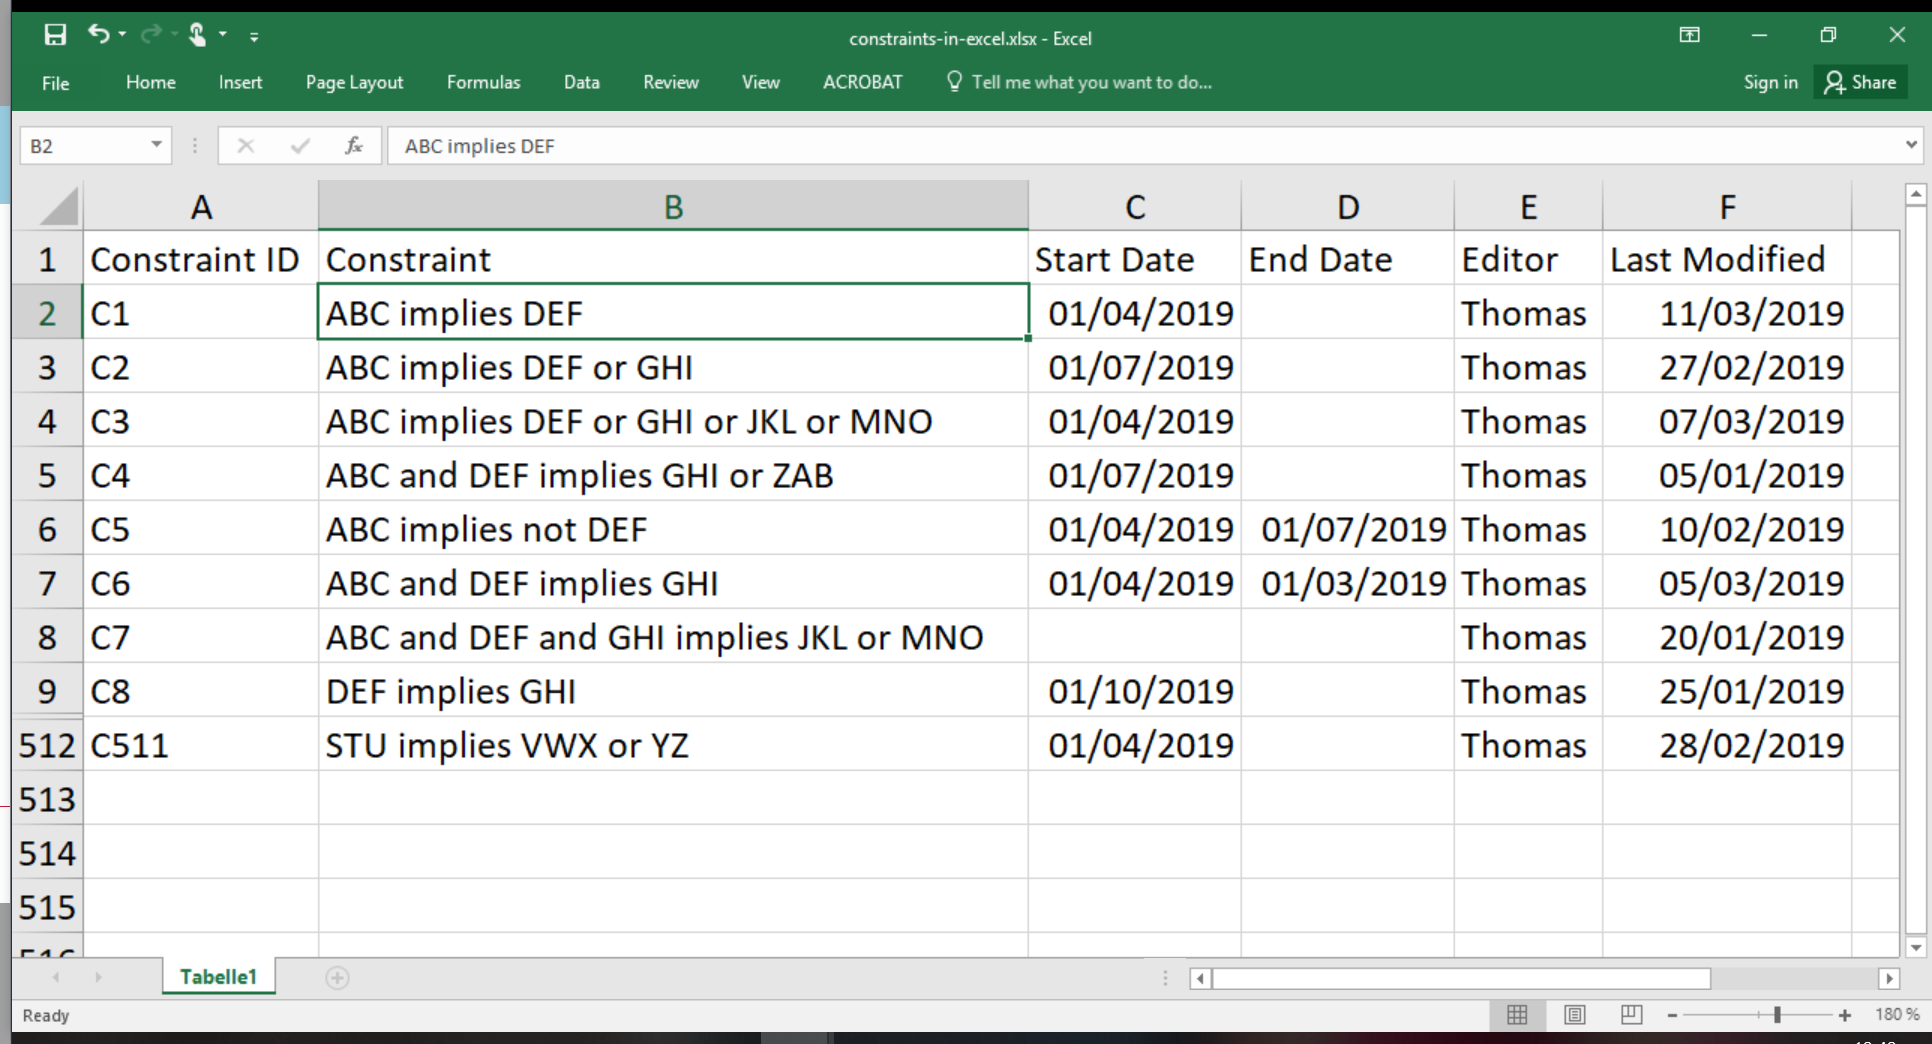
\includegraphics[width=.7\linewidth,trim=10 10 0 10,clip]{constraints-in-excel}
% \end{frame}

\begin{frame}{\myframetitle}
	\myexampletight{Representations of Variability Models}{
		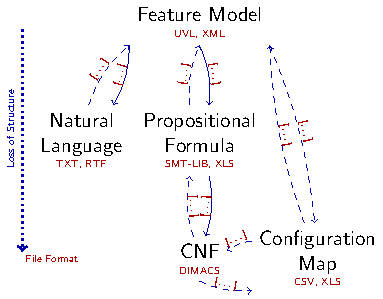
\includegraphics[width=\linewidth]{representations-low-level}

		% describe sat, #sat, allsat
		% describe size of product lines (chico)

		% \myexampletight{Industrial Configuration Spaces \mysource{\evaluatingsharpsatsolvers}}{
		% 	\centering\evaluatingsharpsatsolverslink{\includegraphics[width=\linewidth,page=6,trim=50 210 320 440,clip]{2020/2020-VaMoS-Sundermann}}
		% }

		% feature model of the linux kernel als motivation nutzen, dann recap in testing VL
	}
\end{frame}